\documentclass[12pt,a4paper]{article}

\usepackage{fontspec}
\usepackage{amsmath,amssymb}
\usepackage{graphicx}
\usepackage{booktabs}
\usepackage{hyperref}
\usepackage{xcolor}
\usepackage{listings}
\usepackage[margin=2.5cm]{geometry}
\usepackage{float}
\usepackage{subcaption}

\usepackage{xepersian}
\settextfont[Scale=1.1]{Vazirmatn}
\setlatintextfont{Times New Roman}
\setdigitfont[Scale=1.1]{Vazirmatn}

\usepackage{titlesec}
\titlespacing*{\section}{0pt}{2.5ex plus 1ex minus .2ex}{1.5ex plus .2ex}
\titlespacing*{\subsection}{0pt}{2ex plus 1ex minus .2ex}{1ex plus .2ex}
\titlespacing*{\subsubsection}{0pt}{1.5ex plus 1ex minus .2ex}{.8ex plus .2ex}

\lstset{
  language=Python,
  basicstyle=\ttfamily\scriptsize,
  keywordstyle=\color{blue},
  commentstyle=\color{gray}\itshape,
  stringstyle=\color{red!70!black},
  numbers=left,
  numberstyle=\tiny\color{gray},
  frame=single,
  breaklines=true,
  tabsize=4,
  showstringspaces=false,
}

\hypersetup{
  colorlinks=true,
  linkcolor=blue!60!black,
  urlcolor=blue!60!black,
}

\begin{document}

% عنوان ساده
\begin{center}
{\Large\bfseries گزارش پروژه سوم}\\[0.3cm]
{\large نرم‌افزار ریاضی}\\[0.5cm]
شماره دانشجویی: 40213427\\
تاریخ: تیر ۱۴۰۵
\end{center}

\vspace{1cm}

% ============ بخش ۱ ============
\section{درون‌یابی لاگرانژ و اسپلاین}

نقاط داده‌شده:
$$
(1,1),\ (2,3),\ (3,5),\ (4,8),\ (5,5),\ (6,2)
$$

\subsection{درون‌یابی لاگرانژ}

برای ۶ نقطه، یک چندجمله‌ای درجه ۵ به دست می‌آید. فرمول کلی:
$$
P(x) = \sum_{i=0}^{5} y_i \cdot L_i(x), \qquad L_i(x) = \prod_{\substack{j=0 \\ j\neq i}}^{5} \frac{x - x_j}{x_i - x_j}
$$

کدی که نوشتم، یک تابع \lr{lagrange\_basis} برای محاسبه هر $L_i$ و یک تابع \lr{lagrange\_interp} برای جمع‌بندی دارد:

\begin{latin}
\begin{lstlisting}
def lagrange_basis(i, x, xn):
    L = 1.0
    for j in range(len(xn)):
        if j != i:
            L *= (x - xn[j]) / (xn[i] - xn[j])
    return L

def lagrange_interp(x, xn, yn):
    s = 0.0
    for i in range(len(xn)):
        s += yn[i] * lagrange_basis(i, x, xn)
    return s
\end{lstlisting}
\end{latin}

ضرایب چندجمله‌ای (\lr{np.polyfit}) به دست آمد:
$$
P(x) = 0.175x^5 - 2.9583x^4 + 18.375x^3 - 52.0417x^2 + 68.45x - 31
$$

خطای درون‌یابی در تمام نقاط گره برابر صفر ماشینی بود.

\subsection{اسپلاین مکعبی طبیعی}

برای اسپلاین از کتابخانه \lr{scipy} استفاده کردم. در این روش به جای یک چندجمله‌ای بزرگ، در هر بازه $[x_i, x_{i+1}]$ یک چندجمله‌ای درجه ۳ جداگانه ساخته می‌شود:
$$
S_i(x) = a_i + b_i(x-x_i) + c_i(x-x_i)^2 + d_i(x-x_i)^3
$$

شرایط مرزی طبیعی یعنی $S''$ در دو سر بازه صفر باشد. ضرایب هر بازه از خروجی کد:

\begin{latin}
\begin{lstlisting}[numbers=none]
  [1, 2]: d=-0.1866, c=0.0000, b=2.1866, a=1.0000
  [2, 3]: d= 0.9330, c=-0.5598, b=1.6268, a=3.0000
  [3, 4]: d=-2.5455, c=2.2392, b=3.3062, a=5.0000
  [4, 5]: d= 2.2488, c=-5.3971, b=0.1483, a=8.0000
  [5, 6]: d=-0.4498, c=1.3493, b=-3.8995, a=5.0000
\end{lstlisting}
\end{latin}

\subsection{مقایسه دو روش}

\begin{figure}[H]
  \centering
  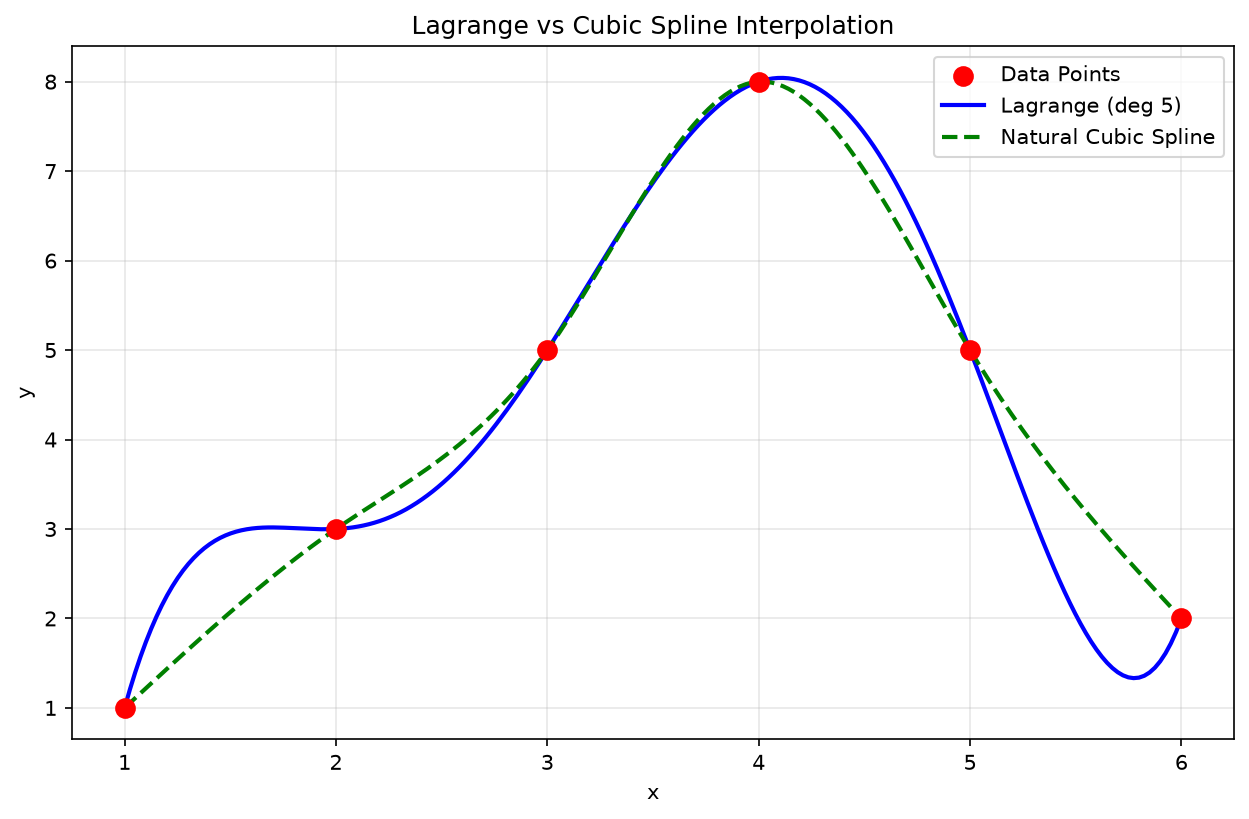
\includegraphics[width=0.85\textwidth]{interpolation_plot.png}
  \caption{مقایسه لاگرانژ و اسپلاین}
\end{figure}

همان‌طور که در نمودار مشخص است، چندجمله‌ای لاگرانژ دقیقاً از همه نقاط عبور می‌کند ولی بین نقاط نوسان زیادی دارد (مثلاً بین $x=4$ و $x=6$ به شدت بالا و پایین می‌رود). اسپلاین مکعبی هم از همه نقاط عبور می‌کند ولی خیلی هموارتر است و نوسان ندارد. برای کاربردهای عملی اسپلاین انتخاب بهتری است.


\newpage
% ============ بخش ۲ ============
\section{تحلیل فایل اکسل}

فایل اکسل داده‌شده شامل زمان اجرای ۳ الگوریتم مختلف برای اندازه‌های ۱۰۰ تا ۶۰۰ کیلوبایت است. کد با \lr{pandas} فایل را می‌خواند و ستون‌ها را به صورت خودکار تشخیص می‌دهد (هیچ داده‌ای دستی وارد نشده):

\begin{latin}
\begin{lstlisting}
df = pd.read_excel(excel_file, engine='openpyxl')
size_col = df.columns[0]
a1, a2, a3 = df.columns[1], df.columns[2], df.columns[3]
\end{lstlisting}
\end{latin}

داده‌های خوانده‌شده:

\begin{table}[H]
\centering
\begin{tabular}{lrrr}
\toprule
\textbf{اندازه} & \textbf{Alg.1} & \textbf{Alg.2} & \textbf{Alg.3} \\
\midrule
100KB & 50 & 200 & 100 \\
200KB & 55 & 220 & 200 \\
300KB & 60 & 240 & 300 \\
400KB & 65 & 260 & 400 \\
500KB & 70 & 280 & 500 \\
600KB & 75 & 300 & 600 \\
\bottomrule
\end{tabular}
\end{table}

\subsection{الف) نمودارها}

\subsubsection{نمودار میله‌ای}
\begin{figure}[H]
  \centering
  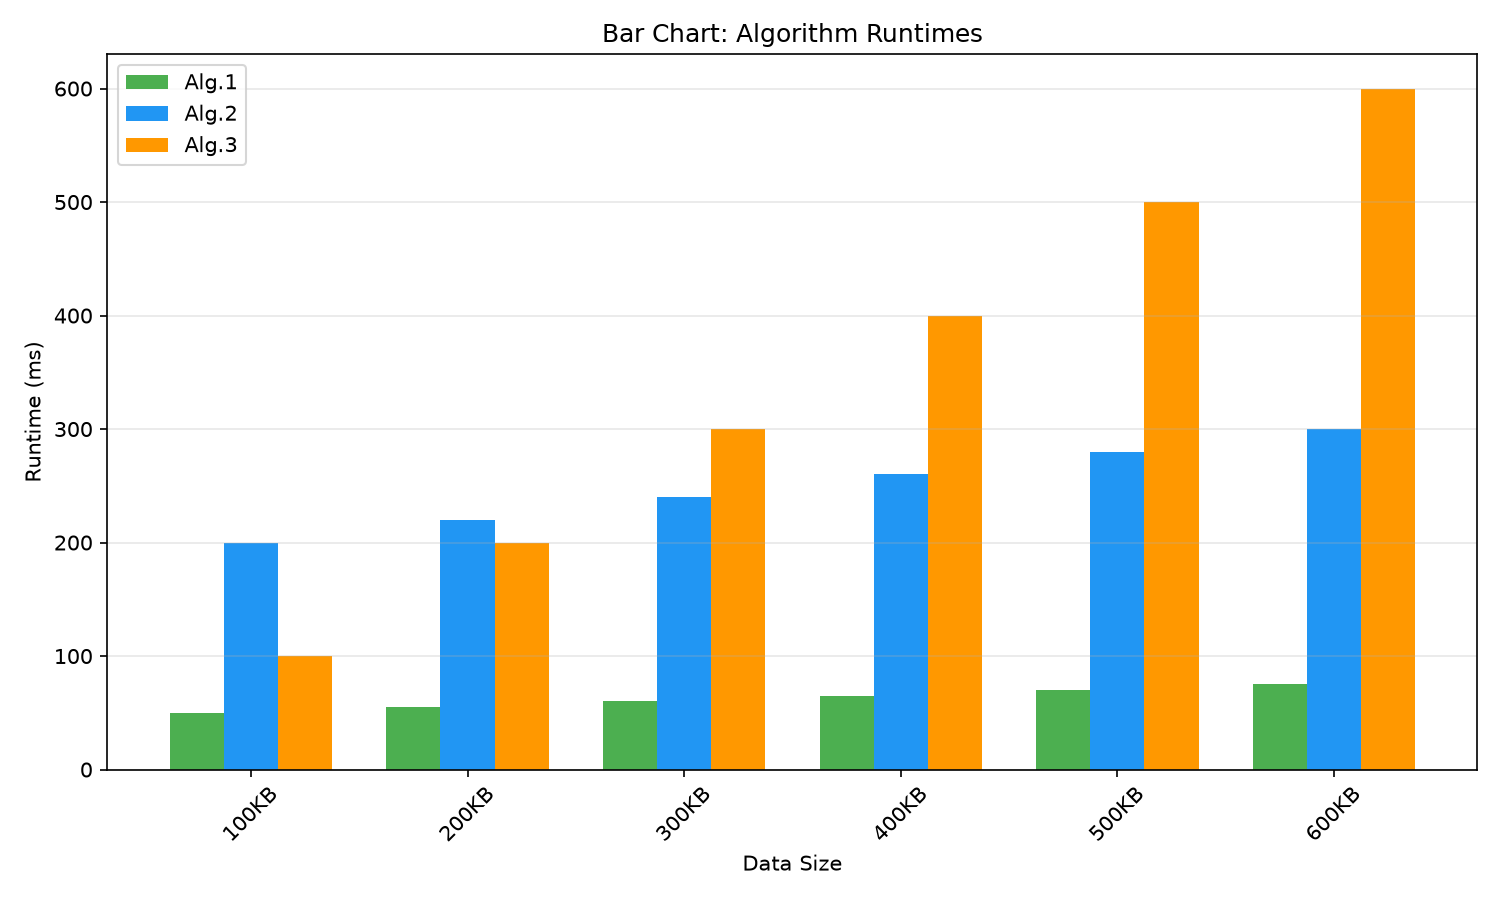
\includegraphics[width=0.8\textwidth]{bar_plot.png}
  \caption{نمودار میله‌ای}
\end{figure}

\lr{(\lr{Alg.1})} سریع‌ترین الگوریتم است و رشد خیلی ملایمی دارد (از ۵۰ تا ۷۵ میلی‌ثانیه). \lr{(\lr{Alg.2})} زمان متوسطی دارد و رشدش یکنواخت و خطی است (از ۲۰۰ تا ۳۰۰). \lr{(\lr{Alg.3})} بیشترین رشد را دارد و زمانش از ۱۰۰ تا ۶۰۰ میلی‌ثانیه می‌رسد.

\subsubsection{نمودار خطی}
\begin{figure}[H]
  \centering
  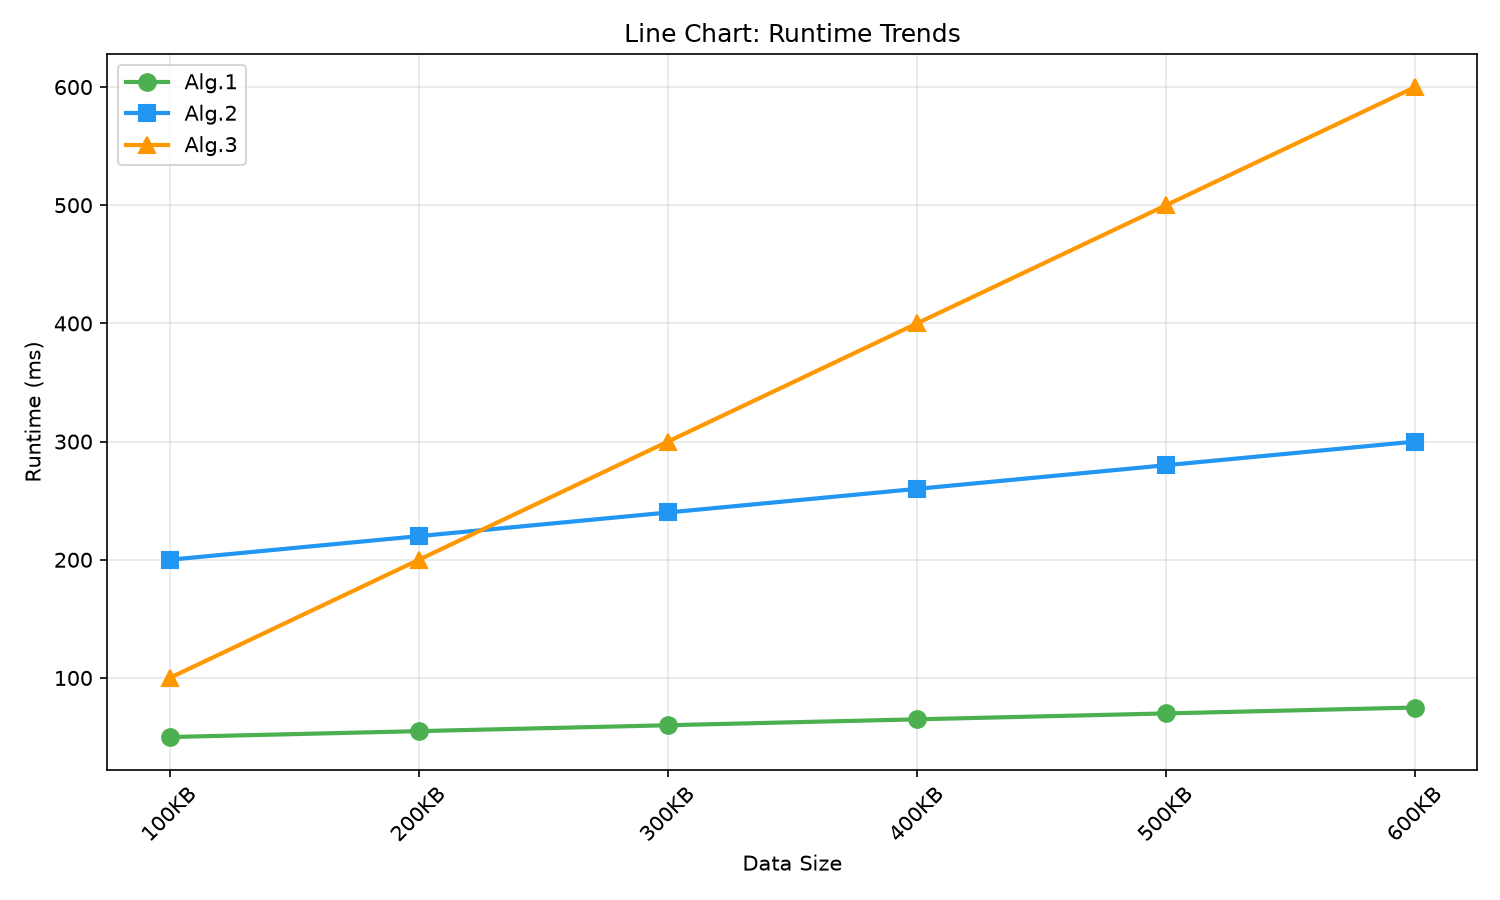
\includegraphics[width=0.8\textwidth]{line_plot.png}
  \caption{نمودار خطی}
\end{figure}

هر سه الگوریتم رفتار خطی دارند ولی شیب‌شان متفاوت است. \lr{(\lr{Alg.3})} بیشترین شیب را دارد و با افزایش داده خیلی سریع رشد می‌کند. \lr{(\lr{Alg.2})} شیب متوسط و یکنواخت دارد (یعنی با دوبرابر شدن داده، زمان حدود ۴۰٪ افزایش می‌یابد). \lr{(\lr{Alg.1})} شیب خیلی کمی دارد و عملاً با افزایش داده رشد نمی‌کند.

\subsubsection{نمودار جعبه‌ای}
\begin{figure}[H]
  \centering
  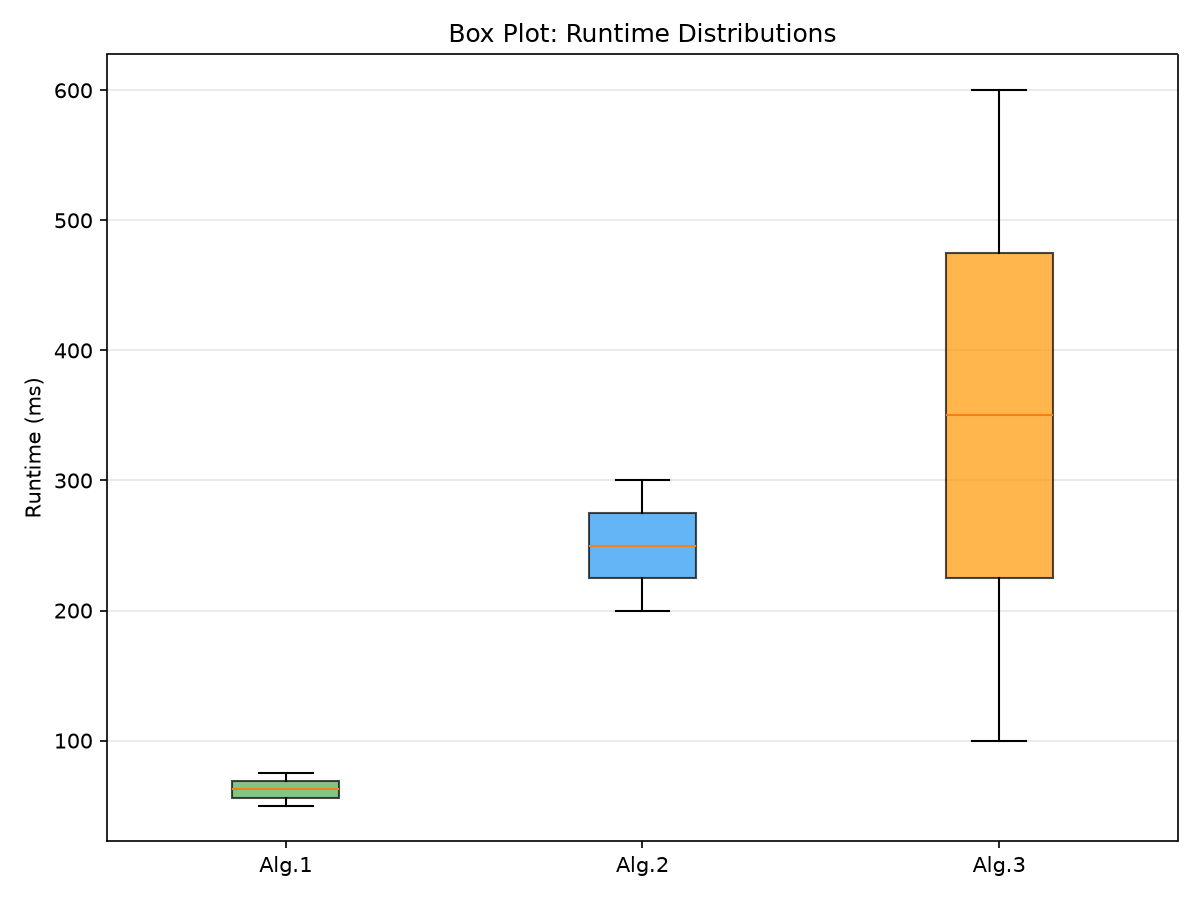
\includegraphics[width=0.65\textwidth]{box_plot.png}
  \caption{نمودار جعبه‌ای}
\end{figure}

\lr{(\lr{Alg.1})} کمترین پراکندگی \lr{(\lr{IQR} \rl{کوچک})} و \lr{(\lr{Alg.3})} بیشترین پراکندگی را دارد. هیچ داده پرتی \lr{(\lr{outlier})} مشاهده نمی‌شود.


\subsection{ب) افزودن داده جدید}

یک سطر جدید \lr{(700KB \rl{با مقادیر 80, 320, 700})} به فایل اکسل اضافه شد. بعد کد \textbf{بدون هیچ تغییری} دوباره اجرا شد و نمودارها به صورت خودکار آپدیت شدند:

\begin{figure}[H]
  \centering
  \begin{subfigure}[b]{0.48\textwidth}
    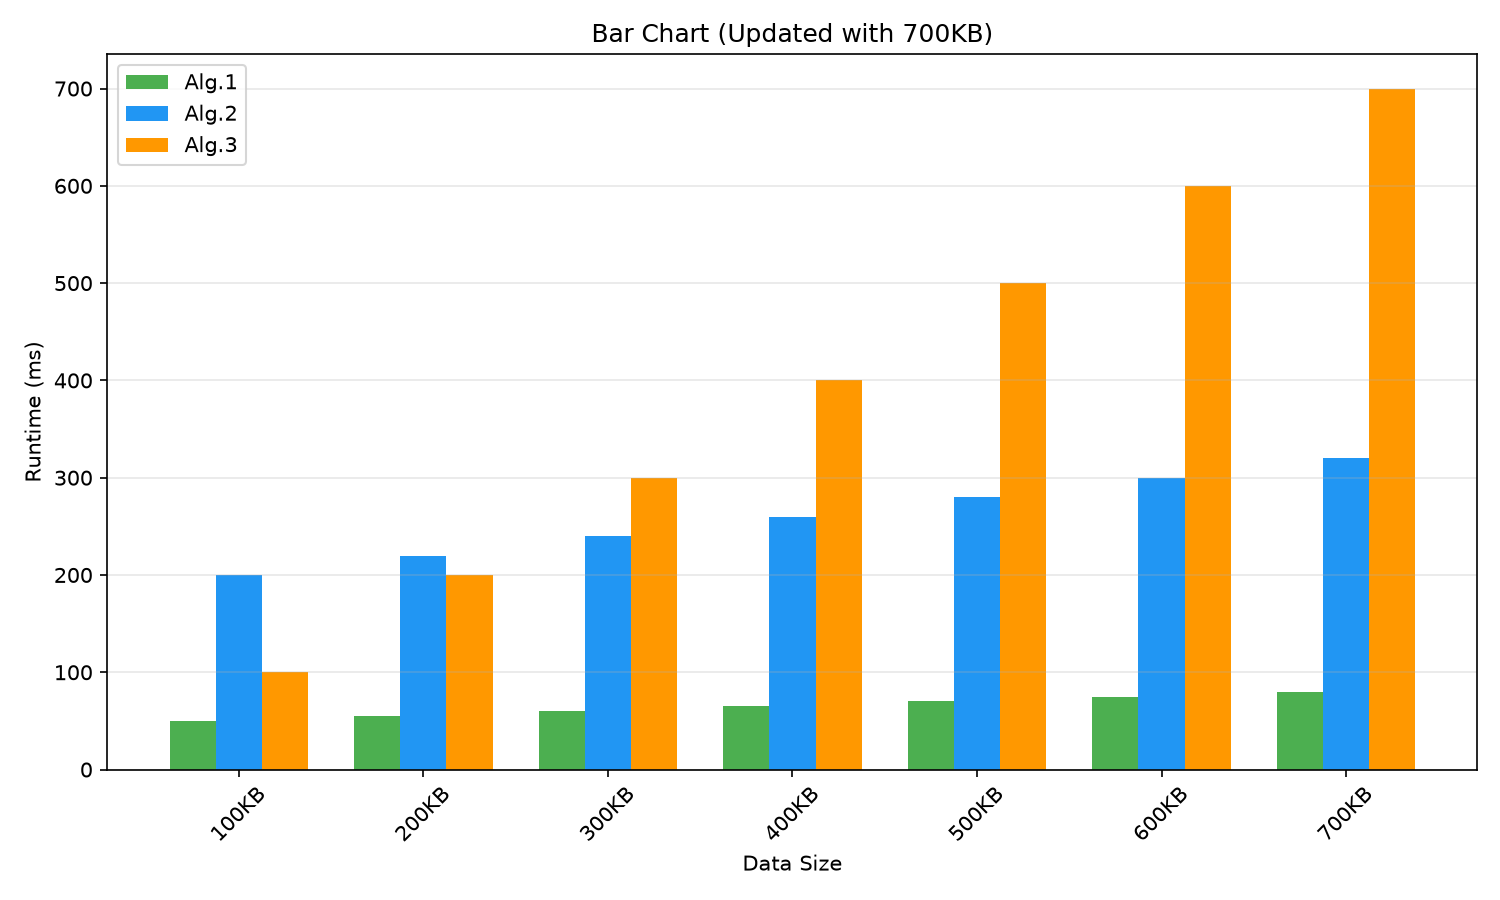
\includegraphics[width=\textwidth]{bar_plot_updated.png}
    \caption{میله‌ای آپدیت‌شده}
  \end{subfigure}
  \hfill
  \begin{subfigure}[b]{0.48\textwidth}
    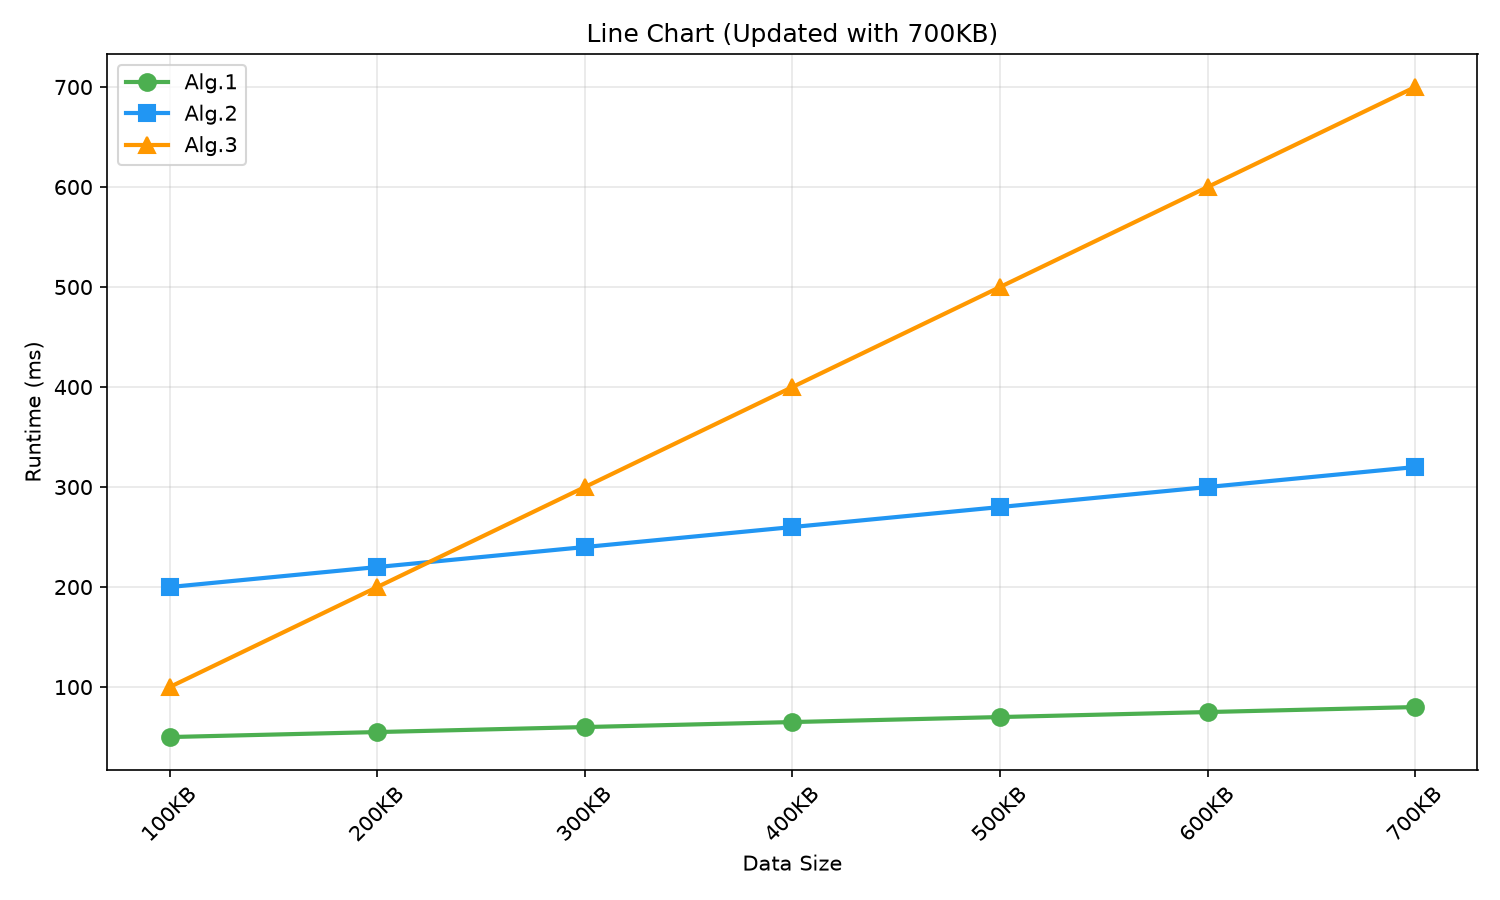
\includegraphics[width=\textwidth]{line_plot_updated.png}
    \caption{خطی آپدیت‌شده}
  \end{subfigure}
  \caption{نمودارهای بعد از اضافه شدن داده 700KB}
\end{figure}

روند قبلی ادامه دارد و داده 700KB هم الگوی خطی را حفظ کرده.

\subsection{ج) میانگین الگوریتم ۲}

مقادیر \lr{Alg.2} برای داده‌های ۱۰۰ تا ۶۰۰ کیلوبایت:
$$
[200, 220, 240, 260, 280, 300] \quad \Rightarrow \quad \text{میانگین} = \frac{1500}{6} = 250 \text{ ms}
$$

\newpage
% ============ بخش ۳ ============
\section{انتگرال‌گیری عددی}

تابع $f(x) = e^x$ در بازه $[0, 1]$. جواب دقیق:
$$
\int_0^1 e^x \, dx = e - 1 \approx 1.718281828459045
$$

\subsection{الف) سیمپسون و ذوزنقه‌ای}

هر دو روش را به صورت ترکیبی پیاده‌سازی کردم. مثلاً کد سیمپسون:

\begin{latin}
\begin{lstlisting}
def simpson(f, a, b, n):
    if n % 2 != 0:
        n += 1
    h = (b - a) / n
    x = np.linspace(a, b, n + 1)
    fx = f(x)
    return (h/3) * (fx[0] + fx[-1] + 4*np.sum(fx[1:-1:2]) + 2*np.sum(fx[2:-2:2]))
\end{lstlisting}
\end{latin}

نتایج سیمپسون:

\begin{table}[H]
\centering
\begin{tabular}{rrr}
\toprule
$n$ & تقریب & خطا \\
\midrule
4 & 1.718318841922 & $3.70 \times 10^{-5}$ \\
8 & 1.718284154700 & $2.33 \times 10^{-6}$ \\
16 & 1.718281974052 & $1.46 \times 10^{-7}$ \\
32 & 1.718281837562 & $9.10 \times 10^{-9}$ \\
64 & 1.718281829028 & $5.69 \times 10^{-10}$ \\
128 & 1.718281828495 & $3.56 \times 10^{-11}$ \\
\bottomrule
\end{tabular}
\end{table}

نتایج ذوزنقه‌ای:

\begin{table}[H]
\centering
\begin{tabular}{rrr}
\toprule
$n$ & تقریب & خطا \\
\midrule
4 & 1.727221904558 & $8.94 \times 10^{-3}$ \\
8 & 1.720518592164 & $2.24 \times 10^{-3}$ \\
16 & 1.718841128580 & $5.59 \times 10^{-4}$ \\
32 & 1.718421660316 & $1.40 \times 10^{-4}$ \\
64 & 1.718316786850 & $3.50 \times 10^{-5}$ \\
128 & 1.718290568083 & $8.74 \times 10^{-6}$ \\
\bottomrule
\end{tabular}
\end{table}

خطای سیمپسون خیلی سریع‌تر کم می‌شود. مثلاً با $n=16$ سیمپسون خطای $10^{-7}$ دارد ولی ذوزنقه‌ای خطای $10^{-4}$ دارد. دلیلش این است که سیمپسون از تقریب درجه ۲ (سهمی) استفاده می‌کند ولی ذوزنقه‌ای از تقریب خطی.

\subsection{ب) انتگرال گوسی-لژاندر}

در این روش به جای نقاط یکنواخت، نقاط بهینه (ریشه‌های چندجمله‌ای لژاندر) انتخاب می‌شوند:
$$
\int_a^b f(x)\,dx \approx \frac{b-a}{2} \sum_{i=1}^{n} w_i \cdot f\!\left(\frac{b-a}{2}\xi_i + \frac{a+b}{2}\right)
$$

\begin{table}[H]
\centering
\begin{tabular}{rrr}
\toprule
تعداد نقاط & تقریب & خطا \\
\midrule
1 & 1.648721270700 & $6.96 \times 10^{-2}$ \\
2 & 1.717896378008 & $3.85 \times 10^{-4}$ \\
3 & 1.718281004373 & $8.24 \times 10^{-7}$ \\
4 & 1.718281827526 & $9.33 \times 10^{-10}$ \\
5 & 1.718281828458 & $6.54 \times 10^{-13}$ \\
6 & 1.718281828459 & $\approx 0$ \\
\bottomrule
\end{tabular}
\end{table}

دقت روش گوسی خیلی بالاتر است. فقط با ۵ نقطه به خطای $10^{-13}$ می‌رسد — خطایی که سیمپسون حتی با ۱۲۸ زیربازه هم بهش نمی‌رسد.

\subsection{مقایسه نهایی}

\begin{table}[H]
\centering
\begin{tabular}{lrr}
\toprule
\textbf{روش} & \textbf{تقریب} & \textbf{خطا} \\
\midrule
سیمپسون ($n=16$) & $1.718281974052$ & $1.46 \times 10^{-7}$ \\
ذوزنقه‌ای ($n=16$) & $1.718841128580$ & $5.59 \times 10^{-4}$ \\
گوسی ($n=5$) & $1.718281828458$ & $6.54 \times 10^{-13}$ \\
دقیق & $1.718281828459$ & --- \\
\bottomrule
\end{tabular}
\end{table}

\begin{figure}[H]
  \centering
  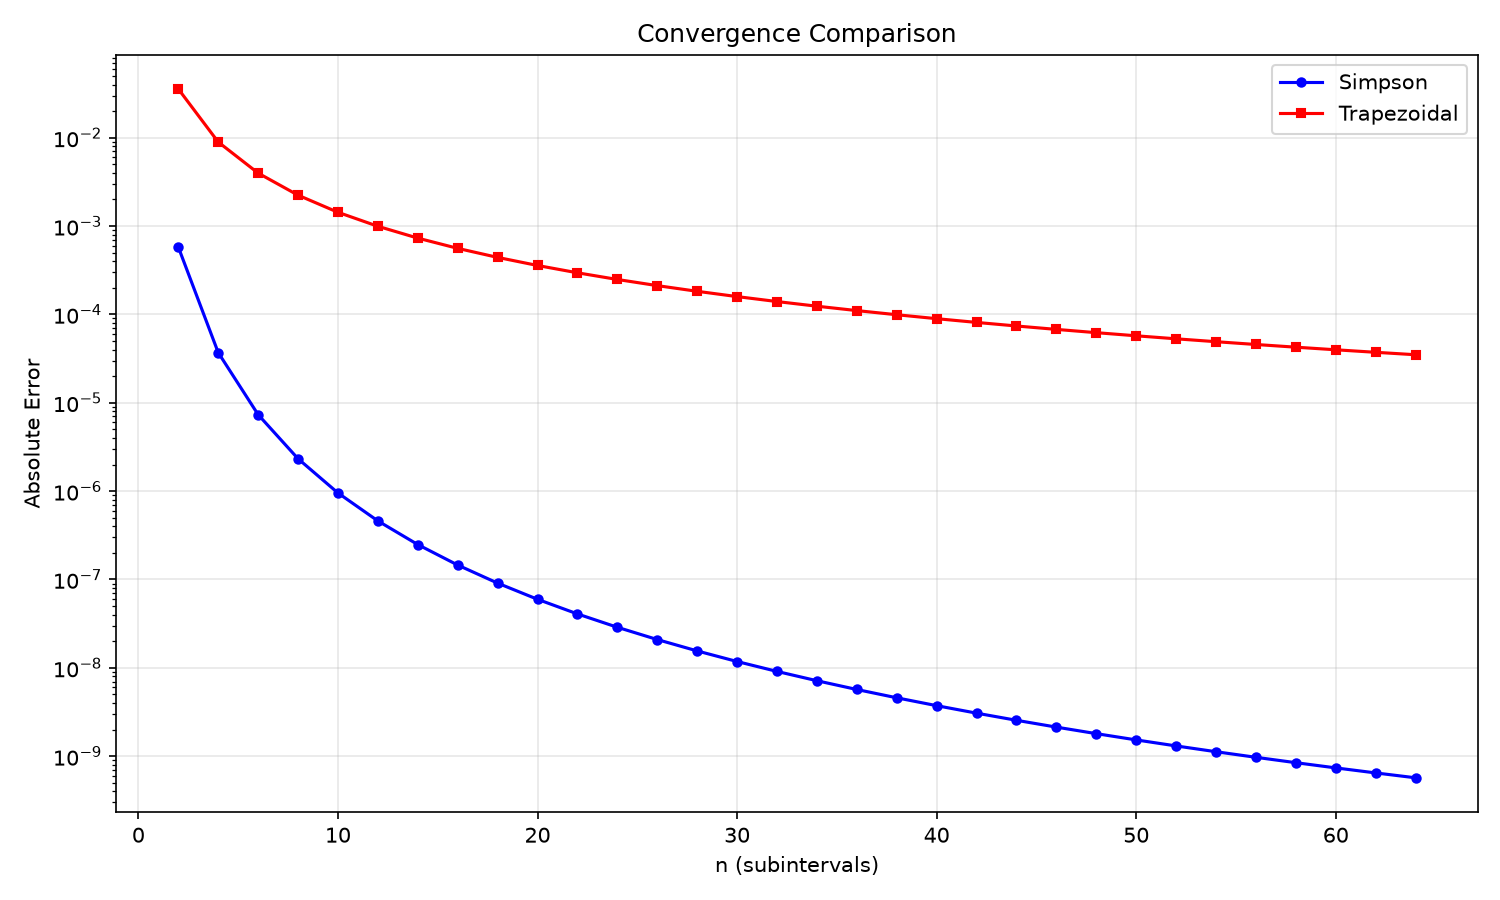
\includegraphics[width=0.8\textwidth]{integration_convergence.png}
  \caption{نمودار همگرایی سیمپسون و ذوزنقه‌ای}
\end{figure}

نمودار همگرایی هم تأیید می‌کند که سیمپسون سریع‌تر همگراست.

\newpage
% ============ بخش ۴ ============
\section{لینک گیت‌هاب}

تمام کدها و گزارش در مخزن عمومی زیر قرار داده شده:

\begin{center}
\url{https://github.com/FarazFazelifar/Mathematical-Software}
\end{center}

\end{document}
